\chapter{\uppercase{Modeling}}

Though the methods presented in this thesis may be useful on a variety of control systems, the primary application used for expositional purposes is bipedal robotic walking.
%
This phenomenon demonstrates two dynamics which operate at different time scales.
%
In particular, nominal motion can be modeled as a continuous dynamics and impact behavior can be treated as a discrete dynamics.
%
The development of the dynamic models for these two dynamics is parallel but a dichotomy arises in the application of constraining forces.

This chapter presents the development of the necessary dynamics for modeling hybrid mechanical systems.


\section{Rigid Body Kinematics}

At its core, the modeling of complex mechanical systems involves a straightforward, if often complicated, application of Newton's Second Law (see \cite{feynman1963}), namely,
that
\begin{align}
  \label{eq:newtons-second}
  F = m a,
\end{align}
which expresses the basic property of physics that applying a force to a massive object induces a particular acceleration.
%
Through the property of superposition, this relationship eventually leads to standard dynamic model of a robot,
\begin{align}
  \M\argsq + \HCor\argsqdq = \B\argsq \, \u
\end{align}
but fundamentally, all physics-based models demonstrate Newton's Second Law.

Consider a three-dimensional rigid body with no contact assumptions; i.e., the body is free to move in space.
%
With the dynamics of the system being dominated by Newton's laws of motion \cite{feynman1963}, the state of the system can be expressed by associating a reference frame to a fix pointed on the body and using coordinates which express the position and orientation of this point with respect to a global frame or the world frame.
%
In three-dimensional space, this transformation between world frame and robot frame can be parameterized with six coordinates: three representing the Euclidean position and three respresenting, for example, an Euler angle--based derivation, namely, the product of three rotation matrices \cite{Baruh98}.
%
The set of all admissible configurations for such a body represents a specific topological space referred to as the {\em special Euclidean group}, $\SE(3)$.
%
This group can be thought of as the Cartesian product of the position and orientation of a body, i.e., $\SE(3) = \R^3 \times \SO(3)$, where $\SO(3)$ is the {\em special orthogonal group} which can be understood as
\begin{align*}
  \SO(n) = \left\{ R \in \R^{n \times n} : R R^T = I, \det R = 1 \right\}.
\end{align*}
For more information on these topological spaces, consult \cite{MLS94}.


Newton's laws eventually lead to the understanding the motion of such a system can be captured by the following dynamic model:
\begin{align}
  \nonumber
  I_{x} \dot{\omega}_{x} + (I_{z} - I_{y}) \omega_{y} \omega_{z} &= M_{x}\\
  \nonumber
  I_{y} \dot{\omega}_{y} + (I_{x} - I_{z}) \omega_{z} \omega_{x} &= M_{y}\\
  \nonumber
  I_{z} \dot{\omega}_{z} + (I_{y} - I_{x}) \omega_{x} \omega_{y} &= M_{z}\\
  \nonumber
  m \dot{v}_{x} &= F_{x},\\
  \nonumber
  m \dot{v}_{y} &= F_{y},\\
  m \dot{v}_{z} &= F_{z},
\end{align}
where linear and angular velocity are represented by $v$ and $\omega$, respectively, and the corresponding accelerations are shown as time derivatives.
%
The applied forces and moments are shown as $F$ and $M$, respectively, and the $I_{x}$, $I_{y}$, and $I_{z}$ terms are the principal moments of inertia about the appropriate axes.
%
As one might guess, this requires that the fixed frame be located at the center of mass and oriented along the principal axes of inertia; it is straightforward to redefine the base coordinates but this form -- the simplest form -- is given for clarity of presentation.

\section{Kinematic Chains}

Typical robots consist of kinematic chains of rigid bodies attached with prismatic or revolute joints, and for simplicity, the resulting dynamics generally has the appropriate contact assumptions baked in to simplify computation, but it is possible to consider each rigid body separately and solve for the appropriate reaction forces which can be applied through $F$ and $M$ to maintain the proper contact (this is typically called the Newton--Euler method \cite{Hollerbach80}).
%
For robotic motion, holonomic constraints act to reduce the allowable motion and, as a consequence, there exists a minimal set of coordinates which can be used to describe a robot's dynamics.
%
This minimal set is referred to as the {\em generalized coordinates}.


\section{Langrangian Formulation}

%\section{Spatial Vector Algebra}
%While a Lagrangian-based approach to modeling is useful for theoretical applications and smaller systems, its shortcomings quickly emerge as systems grow in complexity.
%
%Perhaps more than anything else, this poor scalability stems from the need to successively multiply rotation matrices in symbolic form resulting in progressively larger expressions.
%
%Moreover, as complexity grows, it becomes is increasingly difficult to glean any useful bit of intuition from examining the expressions in symbolic form.

\section{Hybrid Dynamical Systems}

Hybrid dynamical systems are systems which combine continuous and discrete dynamics.
%
By their nature, they provide a useful framework for modeling mechanical systems with impact.
%
Thr combination of dynamics motivates the use of hybrid systems in modeling numerous physical phenomena including bipedal walking, which is the motivating example most pertinent to this thesis.
%

Hybrid dynamical systems have seen widespread use and comprehensive formal development over the years; see, e.g., \cite{BrBoMi98,GoSaTe09,aut_2014_gcsa_01,ScSc00,WGCCM07}.
%
Other frameworks exist for modeling the same physical phenomena such as differential inclusions as discussed in \cite{Filippov88} but hybrid systems methods are becoming increasingly popular.

With the goal of modeling a mechanical system exhibiting both continuous and discrete dynamics, consider a hybrid dynamical system with total energy $\E\argsqdq$ where the coordinates $\q \in \Q$ take values in the {\em configuration space} $\Q$ and the velocities are in the tangent bundle, $T\Q$.
%
For ease of exposition, let the generalized coordinates of the system be represented by $\argsqdq = \x \in \X$ where $\X$ is the state space.
%
The evolution of the system depends on a {\em unilateral constraint}, $h : \R^{n} \to \Rnn$, which can be used to define the {\em guard} or {\em switching surface}.
%
In the case of a bipedal robot with simple foot behavior, a common selection for the unilateral constraint is the height of the swing foot, i.e., $h\argsx = \hnsf\argsq$.
%
By definining unilateral constraints as functions which not be negative and which cause dicrete jumps when the system attempts to cross the zero level set of a function ($h\argsx$), one arrives at a a definition of the {\em domain of admissibility} as
%
\begin{align}
  \label{eq:domain}
  \D &= \left\{ \x \times \R^{n} : h\arx \geq 0 \right\},
\end{align}
%
which describes the admissible states of the system.
%
The boundary at the zero level set of $h\argsx$ naturally gives rise to the switching surface,
%
\begin{align}
  \label{eq:guard}
  \S &= \left\{ \x \in \R^{n} : h\argsx = 0 \mbox{ and } {\dot h}\argsx < 0 \right\}.
\end{align}
%
Using these spaces, an uncontrolled hybrid system can be expressed as
%
\begin{align}
  \HS = \left\{
  \begin{array}{l l}
    \dx = \xf(\x), & \x \in \D \setminus \S,\\
    \xp = \Delta(\xm), & \x \in \S,
  \end{array}\right.
  \label{eq:hsys}
\end{align}
%
where $\xf\arx$ and $\xg\arx$ are smooth vector fields and $\Delta : S \to D \setminus S$ is a smooth map called the reset map (see, e.g., \cite{MoGr05}).
%
Under the action of control effort $\u$, the corresponding hybrid control system has the form
%
\begin{align}
  \HCS = \left\{
  \begin{array}{l l}
    \dx = \xf\arx + \xg\arx \, \u, & \x \in \D \setminus \S,\\
    \xp = \Delta(\xm), & \x \in \S,
  \end{array}\right.
  \label{eq:hcsys}
\end{align}
%
for control values in a set $\U \subseteq \R^{m}$.
%


\section{Solutions to Hybrid Systems}
(cf. \cite{YeMiHo98})

\section{Complex Domain Structure}
Bipedal robotic walking exhibits both discrete and continuous behavior; it is, therefore, natural to model bipedal robots as hybrid systems. A walking gait will be shown to consist of multiple domains---on each domain, the system evolves in a continuous fashion according to a dynamic model derived from a Lagrangian modeling the mechanical system on that domain. This dynamic model will vary depending on which points on the robot are in contact with the ground---having points in contact with the ground introduces kinematic constraints on the system. At a certain point in each domain, i.e., when the contact points change, the model will discretely change to another phase of walking with a different dynamic model and different control. This combination of continuous and discrete phenomena is the fundamental concept underlying hybrid systems.

In this section, a formalism for hybrid systems is introduced and a discussion of how the equations of motion of a robot together with a temporal ordering of discrete events, i.e., change in contact points, completely determine the hybrid model of a system. More specifically, to model bipedal robots, one need only consider the domain breakdown and the Lagrangian on each domain. Details are provided to show how the breakdown can be derived by considering the kinematic constraints imposed on the system throughout the course of a step.


\subsection{Formal Definition of Hybrid Systems}
{\em Hybrid systems} or {\em systems with impulse effects}\cite{GAP01}\xspace have been studied extensively in a wide variety of contexts and have been used to model a wide range of bipedal robotic systems.\cite{GCAS10}\xspace This section introduces a definition of hybrid systems applicable to bipedal walking.

Steady state bipedal walking is naturally periodic with discrete impacts leading to different walking phases. Therefore, when studying walking, one should consider multi-domain hybrid systems with a temporal ordering of events, i.e., systems in which the domain graph is a {\em directed cycle}.

%\begin{figure}[t]
%  \centering
%  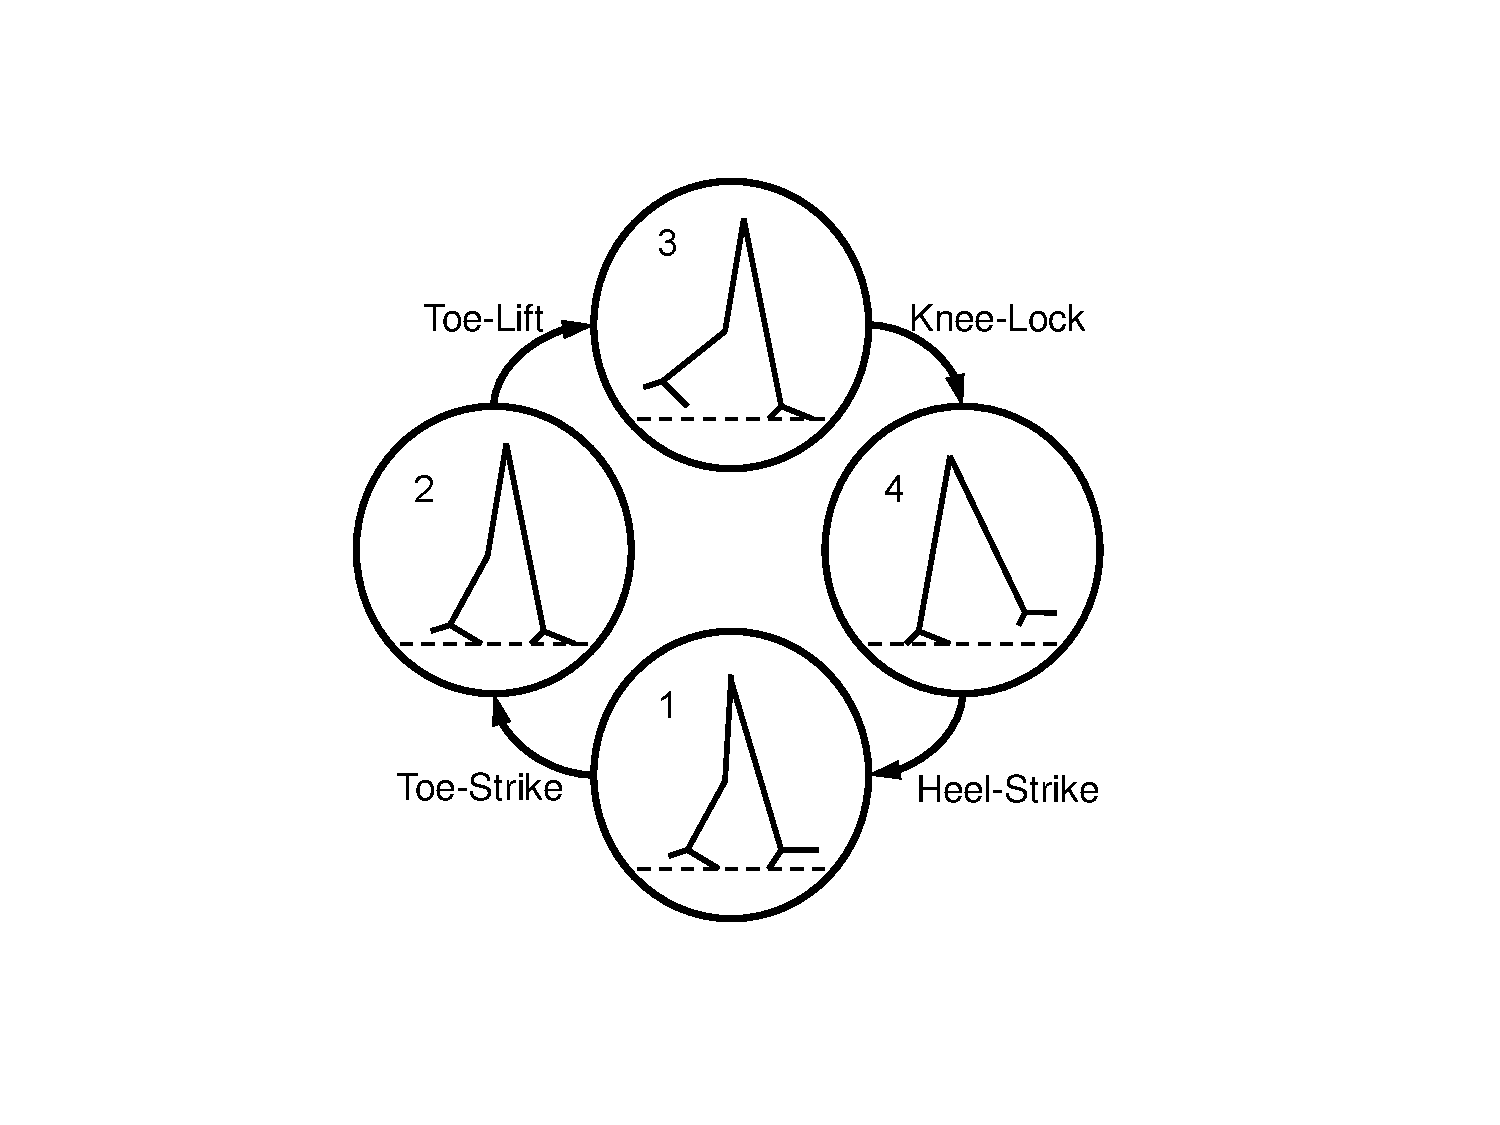
\includegraphics[width=0.7\columnwidth]{figures/domaingraph}
%  \caption{An example of a {\em domain breakdown}---a combination of discrete phases of a walking gait with a specific temporal ordering. The red dots indicate which constraints are enforced in each discrete phase (or domain). The domain labels are selected based on which event causes a given domain to transition to the next.}
%  \label{fig:domaingraph}
%\end{figure}

\begin{definition}
A {\em directed cycle} is a graph $\Gamma = (V, E)$, with $V$ a set of vertices and $E$ a set of edges---for an edge $e \in E$, denote the source by $\sor(e)$ and the target by $\tar(e)$---in which the edges and vertices can be written
\begin{align}
\label{eqn:directedcyclep}
    V &= \left\{v_{1}, v_{2}, \ldots, v_{p}\right\},\\
    E &= \left\{e_{1} = \{v_{1}, v_{2}\}, e_{2} = \{v_{2}, v_{3}\}, \ldots, e_{p} = \{v_{p}, v_{1}\}\right\},
\end{align}
\end{definition}
where $p$ is the number of discrete domains in the corresponding hybrid model.

This concept is illustrated in the following example, which will be used later in this paper:

\begin{exmp} \label{universalgraph}
The domain breakdown pictured in \figref{fig:domaingraph} has an underlying graph that is a directed cycle; the graph is given by $\Gamma_{u} = (V_{u}, E_{u})$. In particular, there are four vertices and four edges with
\begin{align}
    V_u &= \left\{\DA, \DB, \DC, \DD\right\},\\
    E_u &= \left\{\{\DA, \DB\}, \{\DB, \DC\}, \{\DC, \DD\}, \{\DD, \DA\}\right\}.
\end{align}
\end{exmp}

The concept of a directed cycle a fundamental component in the forumulation of multidomain hybrid systems:

\begin{definition} A {\em hybrid control system in a cycle} is a tuple,
\begin{align}
  \HCS = (\Gamma, \D, U, S, \Delta, FG),
\end{align}
\end{definition}
where
\begin{itemize}
  \item $\Gamma = (V,E)$ is a {\em directed cycle},
  \item $\D = \{\D_{v}\}_{v \in V}$ is a set of {\em domains} with $\D_{v} \subseteq \mathcal{X}_{v} \times U_v$ a smooth submanifold, where $\mathcal{X}_{v}$ represents the state space,
  \item $U = \{U_{v}\}_{v \in V}$ with $U_{v} \subseteq \R^{m_{v}}$ a set of admissible controls,
  \item $S = \{S_{e}\}_{e \in E}$ is a set of {\em guards} or {\em switching surfaces}, with $S_{e} \subseteq \D_{\sor(e)}$,
  \item $\Delta = \{\Delta_{e}\}_{e \in E}$ is a set of {\em reset maps}, with $\Delta_{e} : S_{e} \to \mathcal{X}_{\tar(e)}$ a smooth map,
  \item $FG = \{(f_{v}, g_{v})\}_{v \in E}$ with $(f_v,g_v)$ a {\em control system} on $D_{v}$, i.e., $\dot{x} = f_{v}(x) + g_{v}(x) u$ $\forall$ $(x^{T}, u^{T})^{T} \in \D_{v}$.
\end{itemize}
A {\em hybrid system} is a hybrid control system with $U_v = \emptyset$ $\forall$ $v \in V$, e.g., any applicable feedback controllers have been applied, making the system closed-loop:
\begin{align}
  \HS = (\Gamma, \D, S, \Delta, F),
\end{align}
where $F = \{f_{v}\}_{v \in E}$, with $f_{v}$ a (possibly non-autonomous) {\em dynamical system} on $\mathcal{X} \subseteq \D_{v}$, i.e., $\dot{x} = f_{v}(x,t)$.

\subsection{Obtaining Hybrid Systems from Constraints}
The remainder of this section is devoted to discussing how the Lagrangian for a biped, together with a domain breakdown (which determines the constraints at each vertex of the associated cycle), allows one to explicitly construct a hybrid model of the system.  Many details of this construction are only outlined due to space constraints, but more detail is available in the literature.\cite{GCAS10}


%\begin{figure}
%\centering
%  \includegraphics[width=.7 \columnwidth]{figures/bipede_parametrisation_new}
%  \caption{A three-dimensional bipedal robot, together with world ($R_0$), body ($R_b$) and reference ($R_c$) coordinate frames} \label{biped}
%\end{figure}


\subsubsection{General Setup}
Begin with a bipedal robot in either two or three dimensions---the discussions in this paper are applicable to either case. Then construct a Lagrangian for the biped in a general position---specifically, no assumptions are made on ground contact---and then use holonomic constraints to enforce the ground contact conditions given by the domain graph.

\subsubsection{Lagrangians}
Following an existing presentation,\cite{GCAS10}\xspace let $R_{0}$ be a fixed inertial or world frame and let $R_{b}$ be a reference frame attached to the body of the biped with position $p_{b} \in \R^{3}$ and orientation $\phi_{b} \in SO(3)$ where $SO(n)$ represents the special orthogonal group in $n$ dimensions.\cite{CCNPW86}\xspace Let $q_{s} \in Q_{s}$ represent a choice of {\em body} or {\em shape coordinates} for the robot with $Q_{s}$ the configuration space. In this paper, $q_{s}$ represents the relative angles between adjacent links of the robot as shown later in \figref{fig:shapecoords}. The {\em generalized coordinates} are then found by combining the shape coordinates with the position and orientation of the body-fixed frame, $R_{b}$, viz.
\begin{align}
  q = (p_{b}^{T}, \phi_{b}^{T}, q_{s}^{T})^{T} \in Q = \R^{3} \times SO(3) \times Q_{s},
\end{align}
where $Q$ is the generalized configuration space.

The Lagrangian of a bipedal robot, $L : TQ \to \R$, can be stated in terms of the kinetic energy, $K : TQ \to \R$, and the potential energy, $V : Q \to \R$, as:
\begin{align}
  L(q, {\dot q}) = K(q, {\dot q}) - V(q).
\end{align}
The Euler-Lagrange equations can be used to find the equations of motion, which, for robotic systems,\cite{MLS94}\xspace are written:
\begin{align}
  \label{eqn:eom}
  D(q)\ddot{q} + H(q,\dot{q}) = B(q) u
\end{align}
where, here, $D(q)$, the manipulator inertia matrix, and $B(q)$, the torque distribution matrix, only depend on $q$, $u$ is a vector of applied torques, and
\begin{align}
  H(q,{\dot q}) = C(q,{\dot q}) {\dot q} + G(q)
\end{align}
contains terms resulting from the Coriolis effect and gravity terms grouped into a single vector. The matrix $C(q, {\dot q})$ can be found using standard methods.\cite{MLS94}

\subsubsection{Constraints} The continuous dynamics of the system depend on which constraints are enforced at any given time while the discrete dynamics depend on the change in constraints.  Constraints and their enforcement are dictated by the number of contact points between the system and the ground. Specifically, one can define a {\em contact set} $\C = \{c_{1}, c_{2}, \ldots, c_{k}\}$, with each $c_i$ a specific type of foot/ground contact possible in the biped. Assuming that foot contact is restricted to edges parallel to the $y$-axis (i.e., the toe edge or the heel edge)---and this is the case in 2D as in this paper---there are four contact points of interest:
\begin{align}
  \C =  \{\csh, \cst, \cnsh , \cnst\},
\end{align}
where these constraints physically represent the stance heel, stance toe, non-stance heel, and non-stance toe, respectively. The reason for choosing this set of contact points will become clear after data analysis.

\begin{remark}
  In some of the literature, the term non-stance is referred to as swing. This is an artifact of point-foot bipedal models which have only single support and instantaneous double support (at impact). This paper instead uses the term non-stance due to the existence of noninstantaneous double support phases where there are periods with no free swinging behavior. In this case the naming of stance/non-stance legs is arbitrary; in this paper, the stance leg is defined as the leg holding most of the weight of the robot.
\end{remark}

%%%% FIX
%%%% Need to fix the motivation at the end of the preceding paragraph
%%%% Cite domain breakdown submission


%%%% FIX
%%%% Need to treat the following section in a more correct manner, e.g., flat foot vs. toe roll
Contact points introduce {\it holonomic constraints}, $\eta_{c}$ for $c \in \C$, on the system; this vector must be held constant for the contact point to be maintained. To construct these constraints, consider a reference frame $R_{c}$ at the contact point $c$ such that the axis of rotation about this point (either the heel or toe) is along $y$-axis. Let $R_0^c(q)$ be a rotation matrix between reference frames from $R_{0}$ and $R_{c}$. Let $p_{c} : Q \to \R^{3}$ represent the position of the frame and let $v_{c}(q, {\dot q}) = {\dot p}_{c}(q, {\dot q})$ represent the velocity. The body-fixed angular velocity of the frame can then be found:
\begin{align}
  \label{eq:angvelmat}
  \Omega_{c}(q, {\dot q}) &= (R_{0}^{c}(q))^{T} \, \pd{R_{0}^{c}(q)}{q} {\dot q}\\
  \nonumber
  &= \left[\begin{array}{c c c}
      0 & -\omega_{c}^{z}(q, {\dot q}) & \omega_{c}^{y}(q, {\dot q})\\
      \omega_{c}^{z}(q, {\dot q}) & 0 & -\omega_{c}^{x}(q, {\dot q})\\
      -\omega_{c}^{y}(q, {\dot q}) & \omega_{c}^{x}(q, {\dot q}) & 0
    \end{array}\right].
\end{align}
The angular velocity vector
\begin{align}
  \omega_{c}(q, {\dot q}) = (\omega_{c}^{x}(q, {\dot q}), \omega_{c}^{y}(q, {\dot q}), \omega_{c}^{z}(q, {\dot q}))
\end{align}
is dual to the skew-symmetric matrix $\Omega(q, {\dot q})$. Using the linear and angular velocities, the holonomic constraint can be written
\begin{align}
  \eta_{c}(q, {\dot q}) = \left[\begin{array}{c}
      v_{c}(q, {\dot q})\\
      \omega_{c}^{x}(q, {\dot q})\\
      \omega_{c}^{z}(q, {\dot q})
    \end{array}\right] =
  J_{c}(q) {\dot q}.
\end{align}
It is apparent from \eqref{eq:angvelmat} that $v_{c}(q, {\dot q})$ and $\omega_{c}(q, {\dot q})$ are linearly dependent on ${\dot q}$. Furthermore, $v_{c}(q, {\dot q}) = \pd{p_{c}(q)}{q} {\dot q}$ with $p_{c}(q)$ the Cartesian position of the contact point $c$. Therefore, it is possible to find the associated Jacobian matrix: $J_{c}(q) = \pd{\eta_{c}(q, {\dot q})}{{\dot q}}$.

In the case of a 2D biped, as is considered in this paper, the treatment is exactly the same but $\eta_{c}(q, {\dot q}) = (v_{c}^{x}(q, {\dot q}), v_{c}^{z}(q, {\dot q}))^T$. The end result of this choice of coordinates is a holonomic constraint which enforces the condition $\eta_{c}(q, {\dot q}) = \mathrm{constant}$---this fixes the contact point to the ground but allows rotation about the heel or toe depending on the specific type of contact.  It is useful to express the collection of all holonomic constraints in a single matrix $\eta(q, {\dot q}) \in \R^{20 \times 4}$ as:
\begin{align}
  \eta(q, {\dot q}) \!\! = \!\!\! \left[\!\!\begin{array}{c c c c}
      \! \eta_{\sth}(q, {\dot q}) \! & 0 & 0 & 0 \\
      0 & \! \eta_{\stt}(q, {\dot q}) \! & 0 & 0 \\
      0 & 0 & \! \eta_{\nsh}(q, {\dot q}) \! & 0 \\
      0 & 0 & 0 & \! \eta_{\nst}(q, {\dot q}) \!
    \end{array}\!\!\right]
\end{align}

Another class of constraints that is important is the class of {\it unilateral constraints}, $h_{c}(q)$ for $c \in \C$, since they dictate the set of admissible configurations of the system.  Assuming that the knees do not lock, these constraints represent the height of a contact point above the ground, $h_{c}(q) = p_{c}^{z}(q)$, and can be put in the form of a matrix $h(q) \in \R^{4 \times 4}$ in the same manner as holonomic constraints; that is, $h(q) = \mathrm{diag}(h_{\sth}(q), h_{\stt}(q), h_{\nsh}(q), h_{\nst}(q))$.

\subsubsection{Domain Breakdowns}  A domain breakdown is a directed cycle together with a specific choice of contact points on every vertex of the graph. To define this formally, assign to each vertex a binary vector describing which contact points are enforced on each domain.

\gap

\begin{definition}
  \label{def:domainbreakdown}
  Let $\C = \{c_{1}, c_{2}, \ldots, c_{k}\}$ be a set of contact points and $\Gamma$ be a directed cycle.  A {\it domain breakdown} is a binary map $\B : V \to \Z_{2}^{k}$ such that $\B_{i}(v) = 1$ if $c_{i}$ is in contact on $v$ and $\B_{i}(v) = 0$ otherwise.
\end{definition}

\gap

\begin{exmp} \label{ex:domainbreakdown}
  In the case of the graph $\Gamma_{u}$ given in \exmpref{universalgraph} and the set of contact points $\C =  \{\csh, \cst, \cnsh, \cnst\}$, for the graph shown in \figref{fig:domaingraph}, the domain breakdown is formally given by $\B_{u} : V_{u} \to \Z_{2}^{4}$ where $\B_{u}(ts)$, $\B_{u}(tl)$, $\B_{u}(hl)$ and $\B_{u}(hs)$ are given by
  \begin{align}
    \left[ \begin{array}{c} 1  \\ 0 \\ 0 \\ 1 \end{array} \right], \:\:
    \left[ \begin{array}{c} 1  \\ 1 \\ 0 \\ 1 \end{array} \right], \:\:
    \left[ \begin{array}{c} 1  \\ 1 \\ 0 \\ 0 \end{array} \right], \:\:
    \left[ \begin{array}{c} 0  \\ 1 \\ 0 \\ 0 \end{array} \right],
    \label{eq:domainbreakdownvectors}
  \end{align}
  respectively.
\end{exmp}

\subsection{Hybrid System Construction}
It will now be shown that, given a Lagrangian, a directed cycle, and a domain breakdown, a hybrid system can be explicitly constructed.  Since the Lagrangian is intrinsic to the robot being considered, a domain breakdown alone dictates the mathematical model of the biped.

\subsubsection{Continuous Dynamics}
The control system $\dot{x} = f_v(x) + g_v(x)u$ can be explicity constructed through the constraints imposed on each domain by the domain breakdown. For the domain $v \in V$, the imposed holonomic constraints are given by:
\begin{align}
  \eta_{v}(q, {\dot q}) = \eta(q, {\dot q})\B(v),
\end{align}
where the domain breakdown dictates which constraints are enforced. One can calculate the Jacobian matrix used to enforce the constraints by differentiating the holonomic constraint and removing redundancies as follows:
\begin{align}
  J_{v}(q) = \mathrm{Basis}\left( \mathrm{RowSp}\left( \pd{\eta_{v}(q, {\dot q})}{{\dot q}} \right) \right).
\end{align}
By taking a basis for the row space of the Jacobian, redundant constraints are removed so that $J_v(q)$ has full row rank. Using this Jacobian, the constrained dynamic model is given by
\begin{align}
  \label{constraineddynamics}
  D(q){\ddot q} + H(q,{\dot q}) = B(q) u + J_v^T(q) F_v(q, {\dot q}, u).
\end{align}
where $D(q)$, $H(q, {\dot q})$ and $B(q)$ are as in \eqref{eqn:eom} and $F_v(q, {\dot q}, u)$ is a {\em wrench} containing forces and moments expressed in the reference frame $R_c$.\cite{MLS94}\xspace Because the robot is modeled in a generalized position with ground contact enforced through constraints, the matrices $D(q)$, $H(q, {\dot q})$, and $B(q)$ are identical in every domain. To determine the wrench $F_v(q, {\dot q}, u)$, one differentiates the kinematic constraint $J_v(q) {\dot q} = \mathrm{constant}$ to obtain
\begin{align}
  J_{v}(q) {\ddot q} + {\dot J}_{v}(q, {\dot q}) \, {\dot q} = 0
\end{align}
and combine this equation with \eqref{constraineddynamics}. Doing so results in an expression for the wrench $F_v(q, {\dot q}, u)$:
\begin{align}
  \label{eq:wrench}
  \lefteqn{F_{v}(q, {\dot q}, u) = -\left( J_{v}(q) D^{-1}(q) J_{v}^{T}(q) \right)^{-1} }\\
  \nonumber
  &&\left( {\dot J}_{v}(q, {\dot q}) \, {\dot q} + J_{v}(q) D^{-1}(q) \left( B(q) u - H(q, {\dot q}) \right) \right).
\end{align}
This is sometimes referred to in the literature as a Lagrange multiplier.\cite{MLS94}\xspace Combining \eqref{constraineddynamics} and \eqref{eq:wrench} allows one to eliminate $F_{v}(q, {\dot q}, u)$ and obtain the fields associated to the control system $\dot{x} = f_{v}(x) + g_{v}(x) u$. For $x = (q^{T}, {\dot q}^{T})^{T}$,
\begin{align}
  f_{v}(x) \!\! &= \!\!\! \left[\!\!\!\begin{array}{c}
      \dot{q}\\
      D^{-1}(q)\Big( \big(J_{v}^{T}(q) \Xi(q) J_{v}(q) D^{-1}(q) - I \big) H(q, {\dot q}) \\
      \hspace{1cm}- J_{v}^{T}(q) \Xi(q) {\dot J}_{v}^{T}(q, {\dot q}) {\dot q} \Big)
    \end{array}\!\!\!\right],\\
  \label{eqn:controlsystem}
  g_{v}(x) \!\! &= \!\!\! \left[\!\!\!\begin{array}{c}
      0\\
      D^{-1}(q) \big(I - J_{v}^{T}(q) \Xi(q) J_{v}(q) D^{-1}(q) \big) B(q)
    \end{array}\!\!\!\right],
\end{align}
where, for simplicity, $\Xi(q) := \big( J_{v}(q) D^{-1}(q) J_{v}^{T}(q) \big)^{-1}$.

\subsubsection{Discrete Dynamics}
The discrete dynamics consist of the domains, guards and reset maps for a hybrid system and are related to the domain breakdown.

Given a vertex $v \in V$, the domain $\D$ is the set of admissible configurations of the system factoring in both friction and a unilateral constraint. Specifically, from the wrench $F_{v}(q, {\dot q}, u)$, one can ensure that the foot does not slip by considering inequalities on the friction which can be stated in the form:
\begin{align}
  \label{eq:constmu}
  \mu_{v}(q) F_{v}(q, {\dot q}, u) \geq 0,
\end{align}
with $\mu_{v}(q)$ a matrix of friction parameters and constants defining the geometry of the foot.\cite{GCAS10}\xspace Additionally, it has been shown\cite{CBAA09,VBSS90} that the moment produced by the ground is limited; this limitation can be written in the form:
\begin{align}
  \label{eq:constnu}
  \nu_{v}(q) F_{v}(q, {\dot q}, u) \geq 0,
\end{align}
where $\nu_{v}(q)$ depends on the physical parameters and state of the system. Equations \eqref{eq:constmu} and \eqref{eq:constnu} for a given domain can be coupled with the unilateral constraint on the domain, $h_{v}(q) = h(q) \B(v)$, if present, to yield the set of admissible configurations:
\begin{align}
  \label{admissible}
  A_{v}(q, {\dot q}, u) = \left[ \begin{array}{c}
      \mu_{v}(q) F_{v}(q, {\dot q}, u)\\
      \nu_{v}(q) F_{v}(q, {\dot q}, u)\\
      h_{v}(q)
    \end{array} \right] \geq 0.
\end{align}
Thus, the domain is given by
\begin{align}
  \label{eq:domain}
  \D_{v} \! = \! \left\{ \! (q^{T}, \! {\dot q}^{T}, \! u^{T})^{T} \! \in \! TQ \times \R^{m_{v}} : A_{v}(q, {\dot q}, u) \! \geq \! 0 \! \right\}.
\end{align}
The guard is just the boundary of this domain with the additional assumption that the set of admissible configurations is decreasing, i.e., the vector field is pointed outside of the domain, or, for an edge $e = (v, v') \in E$,
\begin{align}
  S_{e} \! = \! \Bigl\{ \!(q^{T}, {\dot q}^{T}, \! u^{T})^{T} \! \in \! TQ \times \R^{m_v} : \ &A_{v}(q, \! {\dot q}, \! u) \! = \! 0 \\
\nonumber
  \mathrm{and} \ &{\dot A}_{v}(q, \! {\dot q}, \! u) \! \leq \! 0 \! \Bigl\}.
\end{align}

The impact equations are obtained by considering the constraints enforced on the subsequent domain; denote the  Jacobian associated to these constraints by $J_{e'}$. For an edge $e = \{v, v'\} \in E$, the post-impact velocity ${\dot q}^+$ is given in terms of the pre-impact velocity ${\dot q}^-$ by balancing angular momentum.\cite{HM94}\xspace Using the Schur complement,\cite{Fuzhen05}\xspace the post-impact velocity can be written:
\begin{align}
  \label{eq:pmap}
  \dot{q}^{+} = P_{e}(q, {\dot q}^{-}) = (I - D^{-1} J_{v'}^T(J_{v'}D^{-1} J_{v'})^{-1} J_{v'}){\dot q}^{-}
\end{align}
with $I$ the identity matrix and $J_{v'}$ the Jacobian matrix associated with the holonomic constraints of the next domain expressed in the coordinates of this domain. The above equation can be used for any discrete transition. For transitions where a contact point strikes the ground, there will be a discrete change in velocities given by \eqref{eq:pmap}. For transitions where a contact point lifts from the ground, there will not be a discrete change; thus $P$ will be the identity map. For the sake of clarification, consider the following example:
\begin{exmp}
  In the case of domain $\DA$, the impact event is toe-strike. A plastic impact occurs with the stance toe, resulting in zero post-impact velocity of the stance toe. The stance heel and non-stance toe both remains on the ground. In order to properly achieve this transition, holonomic constraints on the velocities of stance toe, stance heel, and non-stance toe must be; these constraints lead to the Jacobian matix $J_{\DC}$ which is used in \eqref{eq:pmap}; and, in fact, these are the same constraints present in the domain breakdown in \eqref{eq:domainbreakdownvectors}.
\end{exmp}

In an attempt to simplify the model and obtain biperiodic behavior in the walking, the ``left'' and ``right'' leg must be ``swapped'' at one of the domain transitions; this ``trick'' is common throughout the literature.\cite{GAP01}\xspace This is done with a coordinate transformation (applied to $q$), switching the role of the left and right leg, i.e., a state relabeling procedure, which is included in the calculation of the reset map for that edge. This coordinate transformation can be expressed as a linear map $\mathcal{R}$. For transitions in which no relabeling occurs, $\mathcal{R}_{e} = I$. The reset map is expressed as follows:
\begin{align}
  \Delta_{e}(q, {\dot q}) =
  \left[ \begin{array}{c c}
      \mathcal{R}_{e} & \boldzero\\
      \boldzero & \mathcal{R}_{e}
    \end{array} \right]
  \left[ \begin{array}{c}
      q\\
      P_{e}(q, {\dot q})
    \end{array} \right].
\end{align}
This reset map takes a point on the guard of a domain and maps it into the next domain specified by the domain breakdown.

The end result is that, given a domain breakdown and a bipedal robot, the hybrid model for the biped is completely determined. One of the goals of this paper is to determine the domain breakdowns that humans use and this section demonstrated the importance of the domain breakdown in determining the unique mathematical model of the system.
